% Provenance (never printed): see sources/outline_sources.md (Year 2: the long-term carbon cycle
% and the silicate-weathering thermostat; Palaeozoic glaciations; the Cretaceous greenhouse; the
% PETM; Cenozoic cooling). Reservoirs from IPCC AR6 WG1 Figure 5.12; long-term fluxes after Derry
% (2024); weathering laws after Colbourn and others (2013); Phanerozoic CO2 after Foster and
% others (2017); Phanerozoic temperatures after Judd and others (2024); Cenozoic isotopes from
% CENOGRID (Westerhold 2020); the Eocene--Oligocene transition after Hutchinson and others (2021);
% the PETM after AR6 WG1 chapters 2 and 5. The thermostat model, its curves and every number of
% the exercises and problem from figdata/bachelor-2/deeptime.py and the Book 4 second-writer
% scratch calculator calc/ch26.py.
\chapter{Het klimaat over de geologische tijd}\label{ch:b2:deep-time-climate}

Vijftig miljoen jaar geleden stond er nergens op aarde een ijskap. De lucht bevatte meer dan
duizend delen per miljoen koolstofdioxide, de polen waren veel sterker opgewarmd dan de evenaar, en
bossen van een bijna tropisch soort groeiden op \ang{70}~ZB, door de maanden van de poolnacht heen. Vierendertig
miljoen jaar geleden breidde het ijs zich over Antarctica uit, en het is nooit meer verdwenen. Over de honderden miljoenen
jaren die in de gesteenten zijn vastgelegd, heeft de aarde tussen zulke werelden geschommeld, met ijs en zonder; toch
heeft ze sinds de sneeuwbalperioden van \cref{ch:b2:precambrian-earth} haar oceanen nooit weggekookt en is ze nooit
voorgoed bevroren. Dit hoofdstuk volgt de koolstof die deze klimaten bepaalt, de trage
cyclus die haar tussen de lucht en de gesteenten verplaatst, en de thermostaat die de planeet
bewoonbaar houdt.
% ledger: ipcc:ref-periods, ar6ch2:cenozoic, hutchinson21:eot

\begin{recall}
\textbf{Uit de schoolboeken}: het broeikaseffect en de stralingsforcering; de forcering van
koolstofdioxide groeit met de logaritme van zijn concentratie, \qty{3.93}{W.m^{-2}} per verdubbeling;
de evenwichtsklimaatgevoeligheid, beste schatting \qty{3}{\celsius}; ontgassing; de glaciale cycli
en het Laatste Glaciale Maximum. \textbf{Uit Boek~3}: chemische verwering en de
hydrolyse van silicaten; kleimineralen; carbonaatslibben, de lysocline en de
carbonaatcompensatiediepte. \textbf{Uit eerdere hoofdstukken}: de zwakke jonge zon en de \omterm{def:b2:precambrian-earth:snowball}{sneeuwbalaarde}
(\cref{ch:b2:precambrian-earth}); \omterm{def:b2:phanerozoic-earth:palaeogeography}{paleogeografie} en \omterm{def:b2:phanerozoic-earth:oae}{oceanische anoxische gebeurtenissen}
(\cref{ch:b2:phanerozoic-earth}); \omterm{def:b2:climate-proxies:proxy}{klimaatproxy}'s, $\delta^{18}$O en het \omterm{def:b2:climate-proxies:ice-volume}{ijsvolume-effect}
(\cref{ch:b2:climate-proxies}); orbitale forcering (\cref{ch:b2:orbital-forcing}). De koolstofcyclus,
zijn reservoirs en de verblijftijd behoren tot de biologieboeken, de wet van Arrhenius tot de
scheikundeboeken.
\end{recall}
% ledger: ipcc:erf-2xco2, ipcc:log-co2, ipcc:ecs

\section{De koolstofcyclus op lange termijn}\label{sec:b2:deep-time-climate:cycle}

\subsection*{Reservoirs en fluxen}

\begin{definition}[Koolstofcyclus op lange termijn; carbonaat--silicaatcyclus]\label{def:b2:deep-time-climate:carbon-cycle}
De \emph{koolstofcyclus op lange termijn}\index{koolstofcyclus op lange termijn} is de uitwisseling van koolstof tussen
de oppervlaktereservoirs (atmosfeer, oceaan, biosfeer en bodems) en de vaste aarde: vulkanische en
metamorfe ontgassing, de verwering van gesteenten, en de begraving van carbonaat en organische koolstof in
sedimenten die later gesteente worden of worden gesubduceerd. Haar fluxen zijn klein tegenover de
oppervlaktereservoirs en werken over $10^5$ tot $10^8$ jaar. De
\emph{carbonaat--silicaatcyclus}\index{carbonaat--silicaatcyclus} is haar anorganische deel: koolstofdioxide verlaat de mantel
en de korst bij vulkanen, wordt verbruikt door de verwering van silicaatgesteenten, wordt op de
zeebodem afgezet als carbonaat, en keert terug naar het oppervlak wanneer dat carbonaat wordt gemetamorfoseerd of
gesubduceerd en ontgast.
\end{definition}
% ledger: derry24:fluxes, derry24:subduction, colbourn13:timescale

De biologieboeken volgen koolstof via fotosynthese, ademhaling en de oceaan over jaren tot
eeuwen. Op de tijdschaal van de klimaatgeschiedenis wordt het beeld breder en omvat het de gesteenten. Vóór
het industriële tijdperk bevatte de atmosfeer \qty{591}{PgC} (petagram, of miljarden ton, koolstof);
de oceaan bevatte \num{38700}, bijna alles als opgeloste anorganische koolstof in het intermediaire en
diepe water (\num{37100}); vegetatie, bodems en permafrost bevatten samen \num{3350}. De
actieve oppervlaktereservoirs bevatten samen ongeveer \num{3.5e6} teramol koolstof, zo'n
\qty{42000}{PgC}. Ook de sedimentgesteenten bevatten koolstof, als kalksteen en als organisch materiaal
verspreid door schalies, en ze wisselen die slechts langzaam uit met het oppervlak.
% ledger: ar6ch5:fig512, derry24:residence

Een moderne schatting van de in- en uitstroom, in teramol koolstof per jaar ($\qty{1}{Tmol}$
koolstof is \qty{0.012}{PgC}), ziet er zo uit. Naar de oceaan en de atmosfeer: vulkanische ontgassing bij
mid-oceanische ruggen (1.3), \omterm{def:b2:oceanic-islands:stages}{oceaaneilanden} (1.3), bogen (4.5) en continentale riften (4.2), samen ongeveer 11;
metamorfe ontgassing, 2 tot 4; de verwering van oud carbonaat, 12.3, en de oxidatie van
oude organische koolstof die door erosie is blootgelegd, 8.1, met 2.0 uit geologisch methaan: samen \num{36.7}.
Eruit: carbonaatsedimentatie, ongeveer 26, en de begraving van organische koolstof, ongeveer 16. De twee
kanten zijn in evenwicht binnen hun onzekerheden. Ontgassing uit het binnenste van de aarde levert weinig meer dan een
derde van de instroom (\cref{exo:b2:deep-time-climate:2}); de rest is oude sedimentaire koolstof die opnieuw
de ronde doet. Andere schattingen van de vulkanische flux liggen lager: \qty{0.1}{PgC} per jaar
(ongeveer 8 Tmol) in het mondiale koolstofbudget van het IPCC, of \qty{0.26}{Gt} koolstofdioxide (ongeveer 6
Tmol koolstof) in een overzicht van de US Geological Survey: de vulkanische instroom is bekend tot op een
factor twee.
% ledger: derry24:fluxes, ar6ch5:fig512, usgs:volcanic-co2

\begin{omfigure}
\centering
\begin{tikzpicture}[font=\scriptsize, >={Stealth[length=2mm]},
  box/.style={draw, thick, rounded corners=2pt, align=center, inner sep=4pt},
  up/.style={->, very thick, omThm}, down/.style={<-, very thick, omDef},
  lab/.style={midway, above, sloped, font=\scriptsize}]
% reservoirs: ar6ch5:fig512; active reservoirs derry24:residence; fluxes derry24:fluxes, derry24:subduction
\draw[thick, rounded corners=2pt, fill=blue!6] (-6.3,0) rectangle (6.0,2.6);
\node[anchor=north west, font=\small\bfseries] at (-6.2,2.55) {oppervlaktereservoirs, ongeveer \qty{42000}{PgC}};
\node[box, fill=white] (atm) at (-4.6,1.45) {atmosfeer\\\qty{591}{PgC}};
\node[box, fill=white] (oc) at (0.6,1.45) {oceaan\\\qty{38700}{PgC}};
\node[box, fill=white] (land) at (4.3,1.45) {vegetatie, bodems,\\permafrost \qty{3350}{PgC}};
\draw[->, very thick, omProp] (atm.east) -- (oc.west);
\node[align=center, text=omProp] at (-2.0,0.6) {silicaatverwering 11--12, als bicarbonaat};
\draw[<->, thick, black!50] (oc.east) -- (land.west);
% sedimentary rocks and mantle
\node[box, fill=brown!12, minimum width=5.7cm, minimum height=1.1cm] (rock) at (-3.35,-4.55) {sedimentgesteenten:\\carbonaat en organische koolstof};
\node[box, fill=orange!15, minimum width=3.0cm, minimum height=1.1cm] (mantle) at (4.3,-4.55) {mantel};
% inputs (red, up) and outputs (blue, drawn upwards with the tip at the start)
\draw[up] (-5.7,-4.0) -- node[lab] {carbonaatverwering 12.3} (-5.7,0);
\draw[up] (-4.8,-4.0) -- node[lab] {oud org.\ C geoxideerd 8.1} (-4.8,0);
\draw[up] (-3.9,-4.0) -- node[lab] {geologisch methaan 2.0} (-3.9,0);
\draw[up] (-3.0,-4.0) -- node[lab] {metamorfe ontgassing 2--4} (-3.0,0);
\draw[down] (-1.9,-4.0) -- node[lab] {carbonaatsedimentatie 26} (-1.9,0);
\draw[down] (-1.0,-4.0) -- node[lab] {begraving organisch C 16} (-1.0,0);
\draw[up] (4.3,-4.0) -- node[lab] {vulkanen, riften 11.3} (4.3,0);
\draw[->, very thick, black!70] (rock.east) -- node[above] {subductie 4--6} (mantle.west);
\end{tikzpicture}
\par\smallskip{\small De \omterm{def:b2:deep-time-climate:carbon-cycle}{koolstofcyclus op lange termijn}, met pre-industriële reservoirs uit het mondiale
koolstofbudget van het IPCC en huidige fluxen uit een synthese van 2024, in teramol koolstof per jaar
(\qty{1}{Tmol.yr^{-1}} = \qty{0.012}{PgC.yr^{-1}}). Rood: instroom naar de oppervlaktereservoirs; blauw:
uitstroom. Silicaatverwering verlaat het oppervlak niet: ze verplaatst koolstof uit de lucht naar de
oceaan als bicarbonaat, dat daarna als carbonaatsediment vertrekt.}
\end{omfigure}

Gedeeld door de flux erdoorheen geven de \qty{3.5e6}{Tmol} van de oppervlaktereservoirs een
verblijftijd van koolstof van 8 tot \num{9e4} jaar. Koolstof die de oceaan en de lucht binnenkomt, wordt
binnen zo'n honderdduizend jaar opnieuw begraven, een oogwenk op de schaal van dit hoofdstuk: de
oppervlaktereservoirs volgen de trage in- en uitstroom op de voet, en elk blijvend onevenwicht ertussen
verandert de koolstofdioxide van de lucht.
% ledger: derry24:residence

\subsection*{Verwering van carbonaat en silicaat}

Regen lost koolstofdioxide op en tast gesteenten aan, zoals Boek~3 beschreef. Twee soorten gesteente
gedragen zich heel verschillend. De verwering van een kalksteen neemt één koolstofdioxide uit de lucht en één
koolstof uit het gesteente op in het water; wanneer een marien organisme zijn schaal uit de producten bouwt,
gaat één koolstof terug naar de lucht:
\[
  \ce{CaCO3 + CO2 + H2O -> Ca^{2+} + 2 HCO3^-} , \qquad
  \ce{Ca^{2+} + 2 HCO3^- -> CaCO3 + CO2 + H2O} .
\]
Voor de lucht is de rondgang nul. De verwering van een silicaat, hier geschreven met wollastoniet als
vervanger voor de calciumsilicaten van graniet en basalt, neemt ook koolstofdioxide op, maar brengt
er geen uit het gesteente mee:
\[
  \ce{CaSiO3 + 2 CO2 + H2O -> Ca^{2+} + 2 HCO3^- + SiO2} ,
\]
en het carbonaat dat eruit wordt gebouwd, stuurt er slechts één van de twee terug:
\[
  \ce{CaSiO3 + CO2 -> CaCO3 + SiO2} \quad\text{(netto)} .
\]
Elke mol calcium- of magnesiumsilicaat die op het land verweert, legt zo één mol koolstofdioxide
vast in carbonaatgesteente. Daarom overtreft de carbonaatsedimentatie, ongeveer 26, de carbonaatverwering,
12.3, met ongeveer de 11 tot 12 teramol per jaar die de silicaatverwering verbruikt; en het is de
silicaatverwering, niet die van carbonaat, die de vulkanen over miljoenen jaren in evenwicht houdt.
% ledger: colbourn13:timescale, derry24:fluxes

\section{De thermostaat van de silicaatverwering}\label{sec:b2:deep-time-climate:thermostat}

\subsection*{Een negatieve terugkoppeling}

Silicaatverwering is een chemische reactie, en zoals de meeste verloopt ze sneller wanneer het warm is. Warmte
brengt ook meer regen en meer afvoer, die de producten wegvoeren en vers water naar het
gesteente brengen. De snelheid stijgt dus met de temperatuur; en de temperatuur stijgt met de koolstofdioxide van
de lucht. Een planeet die koolstofdioxide wint, warmt op, verweert sneller en verliest hem weer.

\begin{definition}[Silicaatverweringsthermostaat]\label{def:b2:deep-time-climate:thermostat}
De \emph{silicaatverweringsthermostaat}\index{silicaatverweringsthermostaat} is de negatieve
terugkoppeling tussen het klimaat en de \omterm{def:b2:deep-time-climate:carbon-cycle}{koolstofcyclus op lange termijn}: de verwering van silicaatgesteenten, die
koolstofdioxide uit de atmosfeer naar carbonaatgesteente verplaatst, neemt toe met de temperatuur en de
afvoer, zodat een stijging van de atmosferische koolstofdioxide de snelheid van zijn eigen verwijdering verhoogt en een
daling haar verlaagt. Over $10^5$ tot $10^6$ jaar brengt ze de verwijdering weer in evenwicht met de
ontgassing.
\end{definition}
% ledger: colbourn13:timescale, colbourn13:weathering, hutchinson21:gateways

De temperatuurafhankelijkheid is die van de wet van Arrhenius uit de scheikundeboeken. Met een
activeringsenergie $E_{\text a}$ voor het oplossen van calcium- en magnesiumsilicaten is de verweringsflux bij
een temperatuur $T$ dicht bij een referentie $T_0$
\[
  W = W_0 \exp\Bigl[-\frac{E_{\text a}}{R}\Bigl(\frac1T - \frac1{T_0}\Bigr)\Bigr]
  \approx W_0\, e^{k_T (T - T_0)}, \qquad k_T = \frac{E_{\text a}}{R T_0^2},
\]
omdat $1/T - 1/T_0 \approx -(T - T_0)/T_0^2$. Oplosproeven in het laboratorium geven $E_{\text a} =
\qty{63}{kJ.mol^{-1}}$, en met $T_0 = \qty{288}{K}$ is $k_T = \qty{0.09}{K^{-1}}$: de flux groeit
met ongeveer \qty{9}{\percent} per graad; binnen tien graden van $T_0$ wijkt de benadering
minder dan \qty{3}{\percent} af van de exacte wet (\cref{exo:b2:deep-time-climate:6}). Een veldschatting is
$74 \pm \qty{29}{kJ.mol^{-1}}$, dus de gevoeligheid is onzeker tot op een factor van ongeveer twee. De afvoer
voegt er nog aan toe: met een flux evenredig met $(R/R_0)^{0.65}$ en een afvoer die met
\qty{4.5}{\percent} per graad stijgt, wordt de gecombineerde gevoeligheid $k = 0.09 + 0.65\times0.045 =
\qty{0.119}{K^{-1}}$.
% ledger: colbourn13:weathering
% values: k_run 0.11925 (deeptime.py)

\subsection*{Een eendoosmodel}

Om te zien hoe snel de thermostaat werkt, volgen we de overmaat koolstof $M$ die de oceaan en de atmosfeer
boven een stationaire toestand bevatten. Binnen enkele duizenden jaren na een verstoring hebben de oceaan en de carbonaten van de zeebodem
het grootste deel van een overmaat uit de lucht gehaald; bij een uitstoot van \qty{4000}{PgC} blijft ongeveer
\qty{8}{\percent} in de lucht tot de silicaatverwering die verwijdert. Schrijf $f$ voor die
fractie en $A_0 = \qty{591}{PgC}$ voor de pre-industriële koolstof van de lucht, zodat de koolstofdioxide
van de lucht $C = C_0(1 + fM/A_0)$ is. De opwarming volgt de logaritmische wet met de
klimaatgevoeligheid $S$, $\Delta T = S\log_2(C/C_0)$, en de verwering volgt de exponentiële wet hierboven.
% ledger: colbourn13:timescale, ar6ch5:fig512, ipcc:ecs, ipcc:log-co2

\begin{proposition}[Stationaire toestand en tijdconstante van de thermostaat]\label{prop:b2:deep-time-climate:thermostat}
Laat de overmaat koolstof $M$ van oceaan en atmosfeer veranderen volgens
\[
  \frac{\mathrm dM}{\mathrm dt} = V - W_0\,e^{k\,\Delta T(M)}, \qquad
  \Delta T(M) = S\log_2\Bigl(1 + \frac{fM}{A_0}\Bigr),
\]
waarbij $V$ de ontgassing is en $W_0$ de verwering bij $M = 0$.
\begin{enumerate}
  \item De stationaire toestand heeft $\Delta T^* = \ln(V/W_0)/k$, wat $S$ en $f$ ook zijn.
  \item Als $V = W_0$, neemt een kleine overmaat af als $M(t) = M(0)\,e^{-t/\tau}$ met
        \[
          \tau = \frac{A_0 \ln 2}{f\,k\,S\,W_0} .
        \]
\end{enumerate}
\end{proposition}

\begin{proof}
(1) In een stationaire toestand is $\mathrm dM/\mathrm dt = 0$, dus $W_0e^{k\Delta T^*} = V$ en $\Delta T^* =
\ln(V/W_0)/k$; noch $S$ noch $f$ speelt mee. (2) Dicht bij $M = 0$ is $\log_2(1 + x) \approx x/\ln 2$, dus
$\Delta T \approx SfM/(A_0\ln 2)$ en $e^{k\Delta T} \approx 1 + kSfM/(A_0\ln2)$. Met $V = W_0$
wordt de vergelijking $\mathrm dM/\mathrm dt = -W_0kSfM/(A_0\ln 2) = -M/\tau$, met als oplossing de
exponentiële functie.
\end{proof}

Het eerste resultaat is de kern van de thermostaat. Het legt een temperatuur vast, geen concentratie: als
de vulkanen \qty{20}{\percent} meer ontgassen, komt de aarde $\ln 1.2/0.09 = \qty{2.0}{\celsius}$
warmer tot rust, wat haar klimaatgevoeligheid ook is, en de koolstofdioxide past zich aan tot wat die
opwarming geeft, hier \qty{60}{\percent} meer. Een zwakke verweringsrespons, een kleine $k$, maakt een slechte
thermostaat; een sterke houdt de temperatuur bijna vast.
% values: dT_step 2.026, C_step_ratio 1.597 (deeptime.py)

\begin{example}[De tijdconstante van de thermostaat]\label{ex:b2:deep-time-climate:tau}
Silicaatverwering verbruikt 11 tot \qty{12}{Tmol} koolstof per jaar; neem $W_0 = 11.5\times0.012011
= \qty{0.138}{PgC.yr^{-1}}$. Met $A_0 = \qty{591}{PgC}$, $f = 0.08$, $k = \qty{0.09}{K^{-1}}$ en
$S = \qty{3}{K}$ is
\[
  \tau = \frac{591\times0.693}{0.08\times0.09\times3\times0.138} = \qty{1.37e5}{yr} ,
\]
ongeveer 140 duizend jaar. Met de afvoerfactor, $k = 0.119$, wordt ze korter:
\qty{104}{kyr}.
\end{example}
% ledger: derry24:fluxes, ar6ch5:fig512, colbourn13:timescale, colbourn13:weathering, ipcc:ecs
% values: tau_kT_kyr 137.3, tau_run_kyr 103.6 (deeptime.py)

Het model is grof: de fractie $f$ is geen constante, de chemie van de oceaan is tot één
getal herleid en de verwering tot één globale wet. Modellen met een expliciete oceaan en sedimenten geven
e-foldingtijden van ongeveer \qty{200}{kyr} tot een miljoen jaar. De thermostaat is dus een
regelaar voor de zeer lange termijn: hij doet niets aan het klimaat van de komende paar duizend jaar, en
hij houdt de temperatuur van de aarde binnen grenzen over honderden miljoenen jaren.
% ledger: colbourn13:timescale

\begin{omfigure}
\centering
\begin{tikzpicture}
\begin{groupplot}[group style={group size=2 by 1, horizontal sep=1.6cm},
  omrecord, width=0.47\linewidth, height=5.4cm, xmin=0, xmax=1000,
  xlabel={tijd (\unit{kyr})}, xtick pos=bottom, ytick pos=left,
  tick label style={font=\scriptsize}, label style={font=\small},
  legend style={draw=none, fill=white, font=\scriptsize}]
\nextgroupplot[ymin=0, ymax=5200, ylabel={overmaat koolstof (\unit{PgC})},
  y tick label style={/pgf/number format/1000 sep={\,}},
  legend style={at={(0.97,0.97)}, anchor=north east}]
% computed in figdata/bachelor-2/deeptime.py part pulse; ledger: colbourn13:timescale, colbourn13:weathering, derry24:fluxes, ar6ch5:fig512, ipcc:ecs
\addplot[omThm, line width=1.2pt] table[x=t_kyr, y=M_nl] {figdata/out/bachelor-2-deeptime-pulse.dat};
\addlegendentry{model}
\addplot[black, densely dashed, line width=1.0pt] table[x=t_kyr, y=M_lin] {figdata/out/bachelor-2-deeptime-pulse.dat};
\addlegendentry{gelineariseerd}
\draw[densely dotted] (axis cs:137.3,0) -- (axis cs:137.3,1839);
\node[anchor=west, font=\scriptsize] at (axis cs:145,1400) {$\tau$};
\nextgroupplot[ymin=0, ymax=2.4, ylabel={opwarming (\unit{\celsius})},
  legend style={at={(0.97,0.03)}, anchor=south east}]
% computed in figdata/bachelor-2/deeptime.py part step
\addplot[omThm, line width=1.2pt] table[x=t_kyr, y=dT_nl] {figdata/out/bachelor-2-deeptime-step.dat};
\addlegendentry{model}
\addplot[black, densely dashed, line width=1.0pt] table[x=t_kyr, y=dT_lin] {figdata/out/bachelor-2-deeptime-step.dat};
\addlegendentry{gelineariseerd}
\draw[densely dotted] (axis cs:0,2.026) -- (axis cs:1000,2.026);
\node[anchor=south east, font=\scriptsize] at (axis cs:1000,2.03) {$\ln 1.2/k$};
\end{groupplot}
\end{tikzpicture}
\par\smallskip{\small De eendoosthermostaat met $k = \qty{0.09}{K^{-1}}$ en $S = \qty{3}{K}$.
Links: een uitstoot van \qty{5000}{PgC} op tijdstip nul, geteld nadat de oceaan en de carbonaten hun
deel hebben opgenomen; hij neemt af met de e-foldingtijd $\tau$, eerst iets trager dan de
gelineariseerde wet. Rechts: de ontgassing op tijdstip nul met \qty{20}{\percent} verhoogd; de aarde
warmt op naar de stationaire \qty{2.0}{\celsius} van \cref{prop:b2:deep-time-climate:thermostat}.}
\end{omfigure}
% values: t90_lin_kyr 316.2, t90_nl_kyr 339.9, tau_step_kyr 182.7 (deeptime.py)

De thermostaat verklaart ook de zwakke jonge zon van \cref{ch:b2:precambrian-earth}. De zon wordt
om de paar honderd miljoen jaar enkele procenten helderder, en een aarde met een vaste lucht zou mee opwarmen;
maar warmer betekent snellere verwering, die de koolstofdioxide omlaag haalt tot de temperatuur
terugkeert naar dicht bij waar de ontgassing haar plaatst. De gesteenten van de laatste 420 miljoen jaar tonen precies
dat, zoals de volgende paragraaf laat zien.

\section{Broeikas- en ijskastwerelden}\label{sec:b2:deep-time-climate:states}

\begin{definition}[Broeikas- en ijskasttoestand van het klimaat]\label{def:b2:deep-time-climate:states}
Een \emph{broeikasklimaat}\index{broeikasklimaat} is een lang interval, miljoenen tot
tientallen miljoenen jaren, zonder grote continentale ijskappen, met een hoog gehalte aan atmosferische
koolstofdioxide en een klein temperatuurverschil tussen de evenaar en de polen. Een
\emph{ijskastklimaat}\index{ijskastklimaat} is een lang interval met continentale ijskappen aan één
of beide polen, minder koolstofdioxide en een steile gradiënt van evenaar naar pool. De aarde verkeert sinds
ongeveer \qty{34}{Ma} in een ijskasttoestand.
\end{definition}
% ledger: judd24:phanda, hutchinson21:eot

\subsection*{Koolstofdioxide over 420 miljoen jaar}

Koolstofdioxide van vóór de ijskernen wordt uit proxy's afgelezen: de boorisotopen en organische moleculen
van marien plankton, de huidmondjes van fossiele bladeren, de carbonaatknollen van oude bodems. Een compilatie
van die proxy's uit 2017, tot \qty{420}{Ma} terug en afgevlakt, staat hieronder samen met de vergletsjeringen. Haar
langetermijntrend is een daling van ongeveer \qty{3.4}{ppm} per miljoen jaar, en waarden dicht bij het
pre-industriële niveau verschijnen tweemaal vóór onze eigen tijd: in het Carboon en Perm, en
kort in het late Krijt.
% ledger: foster17:co2, data:b4-foster2017, ar6ch2:deep-co2

\begin{omfigure}
\centering
\begin{tikzpicture}
\begin{axis}[omrecord, omage, width=0.92\linewidth, height=6.4cm, xmin=0, xmax=450, ymode=log,
  ymin=80, ymax=8000, xlabel={ouderdom (\unit{Ma})}, ylabel={koolstofdioxide (\unit{ppm})},
  xtick={0,50,...,400}, ytick={100,200,500,1000,2000,5000}, yticklabels={100,200,500,1000,2000,5000},
  xtick pos=bottom, ytick pos=left, clip=false,
  tick label style={font=\scriptsize}, label style={font=\small}]
% computed in figdata/bachelor-2/deeptime.py part co2; ledger: data:b4-foster2017, foster17:co2, judd24:phanda, hutchinson21:eot, ar6ch5:cenozoic-co2, ics:base.Ordovician, ics:base.Silurian, ics:base.Devonian, ics:base.Carboniferous, ics:base.Permian, ics:base.Triassic, ics:base.Jurassic, ics:base.Cretaceous, ics:base.Paleogene, ics:base.Neogene, ics:colour.Ordovician, ics:colour.Silurian, ics:colour.Devonian, ics:colour.Carboniferous, ics:colour.Permian, ics:colour.Triassic, ics:colour.Jurassic, ics:colour.Cretaceous, ics:colour.Paleogene, ics:colour.Neogene
\fill[blue!12] (axis cs:445.21,80) rectangle (axis cs:443.07,8000);
\fill[blue!12] (axis cs:371.1,80) rectangle (axis cs:298.89,8000);
\fill[blue!12] (axis cs:34,80) rectangle (axis cs:0,8000);
\addplot[name path=hi, draw=none, forget plot] table[x=age, y=hi68] {figdata/out/bachelor-2-deeptime-co2.dat};
\addplot[name path=lo, draw=none, forget plot] table[x=age, y=lo68] {figdata/out/bachelor-2-deeptime-co2.dat};
\addplot[omDef!25, forget plot] fill between[of=hi and lo];
\addplot[omDef, line width=1.2pt] table[x=age, y=co2] {figdata/out/bachelor-2-deeptime-co2.dat};
\addplot[black!60, densely dashed] coordinates {(0,278) (450,278)};
\node[anchor=south west, font=\scriptsize, text=black!70] at (axis cs:440,280) {pre-industrieel};
\node[anchor=north west, font=\scriptsize, text=blue!60!black, align=left] at (axis cs:442,7600) {Laat-\\Ordovicium};
\node[anchor=north, font=\scriptsize, text=blue!60!black, align=center] at (axis cs:335,7600) {laat-paleozoïsche\\ijstijd};
\node[anchor=north, font=\scriptsize, text=blue!60!black, align=center] at (axis cs:17,7600) {cenozoïsch\\ijs};
\foreach \a/\b/\c in {450/443.1/icsOrdovician, 443.1/419.62/icsSilurian, 419.62/358.86/icsDevonian, 358.86/298.9/icsCarboniferous,
  298.9/251.902/icsPermian, 251.902/201.4/icsTriassic, 201.4/143.1/icsJurassic,
  143.1/66/icsCretaceous, 66/23.04/icsPaleogene, 23.04/0/icsNeogene} {
  \edef\tmp{\noexpand\fill[\c] (axis cs:\a,80) rectangle (axis cs:\b,95);}\tmp}
\node[font=\tiny] at (axis cs:431.4,87) {S};
\node[font=\tiny] at (axis cs:389.2,87) {D};
\node[font=\tiny] at (axis cs:328.9,87) {C};
\node[font=\tiny] at (axis cs:275.4,87) {P};
\node[font=\tiny] at (axis cs:226.7,87) {T};
\node[font=\tiny] at (axis cs:172.3,87) {J};
\node[font=\tiny] at (axis cs:104.6,87) {K};
\node[font=\tiny] at (axis cs:44.5,87) {Pg};
\end{axis}
\end{tikzpicture}
\par\smallskip{\small Atmosferische koolstofdioxide over de laatste 420 miljoen jaar: de afgevlakte aanpassing
(lijn) aan een compilatie van proxyschattingen, met haar band van \qty{68}{\percent}, op een logaritmische
schaal. Blauwe banden: de Hirnantiaanse vergletsjering van het Laat-Ordovicium; de laat-paleozoïsche ijstijd,
van haar eerste glaciale afzettingen in het allerlaatste Devoon tot haar grootste ijsuitbreiding aan het einde van het
Carboon; het cenozoïsche ijs sinds \qty{34}{Ma}. De balk onderaan toont de perioden.}
\end{omfigure}

Over dezelfde 420 miljoen jaar werd de zon ongeveer \qty{4}{\percent} helderder, zo'n
\qty{50}{W.m^{-2}} op de afstand van de aarde en \qty{9}{W.m^{-2}} forcering eenmaal gespreid over de
bol en gecorrigeerd voor het albedo. De daling van koolstofdioxide van ongeveer \qty{1400}{ppm} naar de
pre-industriële waarde heft die bijna precies op (\cref{exo:b2:deep-time-climate:7}): in termen van
forcering is de aarde 420 miljoen jaar lang binnen enkele watt per vierkante meter van vandaag gebleven,
en haar ijskasttoestanden kwamen wanneer de gecombineerde forcering van koolstofdioxide en zon onder ongeveer 1
tot \qty{2}{W.m^{-2}} zakte. De auteurs van de compilatie schrijven de compensatie toe aan de terugkoppeling van de
silicaatverwering en de verspreiding van landplanten, waarvan de wortels en bodems de verwering versnellen.
% ledger: foster17:co2, data:b4-foster2017, ipcc:erf-2xco2

\subsection*{Paleozoïsche ijstijden}

Een reconstructie van de globaal gemiddelde oppervlaktetemperatuur uit 2024, die proxygegevens
met klimaatmodellen combineert, plaatst het bereik van het Fanerozoïcum tussen \qty{11}{\celsius}, in de glaciale tijden van
het late Pleistoceen, 129 tot 11.7 duizend jaar geleden, en \qty{36}{\celsius}, in het Turonien, 94 tot \qty{89}{Ma} geleden.
Haar warme en koude intervallen volgen de vergletsjeringen die door tillieten en gekraste rotsvloeren zijn vastgelegd.
% ledger: judd24:phanda

De laat-ordovicische vergletsjering, in het Hirnantien (445.2 tot \qty{443.1}{Ma}), spreidde ijskappen
uit over Gondwana, waarvan een groot deel dicht bij de zuidpool lag (\cref{ch:b2:phanerozoic-earth}), en
viel samen met een van de vijf grote uitstervingen. Haar globaal gemiddelde temperatuur, ongeveer
\qty{21}{\celsius} in de reconstructie, is warmer dan die van latere vergletsjeringen: het uitgestrekte
\omterm{def:b2:wilson-cycle:supercontinent}{supercontinent} maakte zijn binnenland toch koud genoeg voor ijskappen. De laat-paleozoïsche ijstijd is
de langste van het Fanerozoïcum: haar eerste glaciale afzettingen dateren uit het allerlaatste Devoon, haar koudste globale
temperaturen uit het Serpukhovien, ongeveer 330 tot \qty{323}{Ma}, en haar grootste uitbreiding
van ijs uit het einde van het Carboon, 307 tot \qty{299}{Ma}. Ze valt samen met de lage
koolstofdioxide van het Carboon en Perm, die de auteurs van de compilatie verbinden met een zwakkere vulkanische
flux of een sterkere verwering terwijl Pangea werd samengevoegd en zijn gebergten hoog stonden.
% ledger: judd24:phanda, ar6ch2:deep-co2, foster17:co2, ics:base.Silurian

\subsection*{Het broeikasklimaat van het Krijt}

De warmste tijd van de reconstructie is het midden-Krijt, de tijd van de hoge zeespiegel en de
\omterm{def:b2:phanerozoic-earth:oae}{oceanische anoxische gebeurtenissen} van \cref{ch:b2:phanerozoic-earth}. De schattingen van koolstofdioxide ervoor
zijn raadselachtig: de compilatie hierboven geeft zo'n 450 tot \qty{860}{ppm} tussen 100 en
\qty{90}{Ma}, en de reconstructie uit 2024 vindt een mediaan van ongeveer \qty{775}{ppm} voor haar heetste
intervallen, lager dan haar temperaturen doen vermoeden. Of koolstofdioxide en temperatuur toen echt uit elkaar
gingen, of de proxy's de lucht van het Krijt verkeerd lezen, is een open vraag; de auteurs noemen het het ``mesozoïsche
raadsel''.
% ledger: judd24:phanda, data:b4-foster2017

\section{Het Cenozoïcum: van hete broeikas naar ijskast}\label{sec:b2:deep-time-climate:cenozoic}

De beste registratie van de laatste 66 miljoen jaar zit in de schalen van benthische foraminiferen, geboord uit
de diepzeebodem. Hun $\delta^{18}$O stijgt wanneer het diepe water afkoelt en wanneer ijskappen de
lichte isotoop op het land opslaan (\cref{ch:b2:climate-proxies}). De figuur hieronder toont de
referentiereeks die in 2020 uit diepzeeboorkernen werd opgebouwd, gemiddeld over \qty{100}{kyr}.
% ledger: data:b4-cenogrid, ar6ch2:cenozoic

\begin{omfigure}
\centering
\begin{tikzpicture}
\begin{axis}[omrecord, omage, width=0.92\linewidth, height=6.4cm, xmin=0, xmax=67,
  ymin=-1.2, ymax=5.6, y dir=reverse, xlabel={ouderdom (\unit{Ma})},
  ylabel={benthische $\delta^{18}$O (\unit{\permil})}, xtick={0,10,...,60},
  xtick pos=bottom, ytick pos=left, clip=false,
  tick label style={font=\scriptsize}, label style={font=\small}]
% computed in figdata/bachelor-2/deeptime.py part ceno; ledger: data:b4-cenogrid, ar6ch2:cenozoic, ar6ch5:cenozoic-co2, hutchinson21:eot, ipcc:ref-periods, ar6ch5:petm
\fill[omThm!15] (axis cs:53,-1.2) rectangle (axis cs:49,5.6);
\fill[omThm!15] (axis cs:16.9,-1.2) rectangle (axis cs:14.7,5.6);
\addplot[black!45, line width=0.4pt] table[x=age, y=d18O] {figdata/out/bachelor-2-deeptime-ceno.dat};
\addplot[omDef, line width=1.3pt] table[x=age, y=d18O_lt] {figdata/out/bachelor-2-deeptime-ceno.dat};
\draw[omThm, thick, ->] (axis cs:55.85,-0.7) -- (axis cs:55.85,-1.15);
\node[anchor=south, font=\scriptsize, text=omThm] at (axis cs:55.85,-1.15) {PETM};
\node[anchor=north, font=\scriptsize, text=omThm] at (axis cs:51,4.6) {EECO};
\node[anchor=north, font=\scriptsize, text=omThm] at (axis cs:15.8,0.6) {MCO};
\draw[blue!60!black, densely dashed] (axis cs:33.9,-1.2) -- (axis cs:33.9,5.6);
\node[anchor=south west, font=\scriptsize, text=blue!60!black, align=left] at (axis cs:33.6,4.4)
  {Antarctisch ijs\\vanaf \qty{34}{Ma}};
\draw[blue!60!black, densely dashed] (axis cs:2.7,-1.2) -- (axis cs:2.7,5.6);
\node[anchor=north west, font=\scriptsize, text=blue!60!black, align=left] at (axis cs:2.5,-0.9)
  {noordelijke\\ijskappen};
\node[anchor=south west, font=\scriptsize, align=left] at (axis cs:66.3,5.45) {kouder, meer ijs $\downarrow$};
\end{axis}
\end{tikzpicture}
\par\smallskip{\small Benthische $\delta^{18}$O van diepzeeforaminiferen over het Cenozoïcum, uit de
referentiereeks CENOGRID: gemiddelden over \qty{100}{kyr} (grijs) en de langetermijnafvlakking van de dataset
(blauw). De as is omgekeerd, zodat kouder en ijziger omlaag ligt. Gearceerd: het Klimaatoptimum van het Vroeg-Eoceen
(EECO) en het Klimaatoptimum van het Mioceen (MCO); gestreept: het begin van de Antarctische
ijskap en de grote opmarsen van de noordelijke ijskappen.}
\end{omfigure}

Van rechts naar links gelezen vertelt de reeks vier hoofdstukken. Het vroege Cenozoïcum warmde op, via het
\omterm{def:b2:deep-time-climate:petm}{Paleoceen--Eoceen Thermisch Maximum}, tot het Klimaatoptimum van het Vroeg-Eoceen, 53 tot \qty{49}{Ma}, toen
de globale temperatuur 10 tot \qty{18}{\celsius} boven die van 1850--1900 lag (\emph{middelgroot
vertrouwen}, in de taal van het IPCC) en koolstofdioxide tussen 1150 en \qty{2500}{ppm}.
Er volgde een lange afkoeling, onderbroken bij de overgang van Eoceen naar Oligoceen, ongeveer \qty{34}{Ma}, door een
sprong van ongeveer \qty{1.5}{\permil} in $\delta^{18}$O: de eerste grote ijskap op Antarctica, met een
afkoeling van de diepe oceaan in de orde van \qty{2}{\celsius}. Het Klimaatoptimum van het Mioceen, 16.9 tot
\qty{14.7}{Ma}, bracht de warmte terug, 4 tot \qty{10}{\celsius} boven 1850--1900 bij 400 tot
\qty{600}{ppm}. Na het midden-Plioceen, de laatste keer dat koolstofdioxide dicht bij het huidige niveau van 360 tot
\qty{420}{ppm} stond, daalde het met zo'n \qty{30}{ppm} per miljoen jaar, en vanaf \qty{2.7}{Ma} groeiden ijskappen
duurzaam op het noordelijk halfrond: de glaciale cycli van \cref{ch:b2:orbital-forcing} begonnen.
% ledger: ipcc:mpwp-eeco, ar6ch2:deep-co2, ipcc:ref-periods, ar6ch2:mco, ar6ch2:mco-co2, hutchinson21:eot, ar6ch5:cenozoic-co2, ipcc:likelihood

Over de hele laatste 50 miljoen jaar daalde koolstofdioxide met ongeveer \qty{16}{ppm} per miljoen
jaar. Het IPCC noemt de oorzaak onzeker, mogelijk een onevenwicht tussen vulkanische ontgassing en de
twee putten op lange termijn, de begraving van organische koolstof en de silicaatverwering. Een drempel van 750 tot
\qty{1000}{ppm} is gemodelleerd voor de groei van permanente ijskappen op Antarctica; de laatste keer dat
koolstofdioxide zo hoog als \qty{1000}{ppm} stond, was vlak vóór de overgang.
% ledger: ar6ch5:cenozoic-co2, ar6ch2:deep-co2

\begin{dated}{2023}
In 2023 publiceerde een consortium van onderzoekers een gecontroleerde compilatie van alle schattingen van cenozoïsche
koolstofdioxide die toen waren gepubliceerd. In haar reconstructie piekte koolstofdioxide bij ongeveer \qty{1600}{ppm} rond
\qty{51}{Ma}; het ontstaan van de Antarctische ijskap, bij ongeveer \qty{33.9}{Ma}, kwam bij \qty{720}{ppm}; tegen
\qty{32}{Ma} was het gedaald tot \qty{550}{ppm}; het Midden-Mioceen, ongeveer \qty{16}{Ma}, was de laatste
keer dat het hoger bleef dan nu; en het zakte onder \qty{270}{ppm} bij \qty{2.6}{Ma}, toen de aarde
haar huidige toestand met ijs aan beide polen binnenging. Gelezen tegenover de temperatuur geeft de kromme een
\emph{aardsysteemgevoeligheid} --- de opwarming per verdubbeling zodra ijskappen en vegetatie hebben
gereageerd --- van ongeveer \qty{8}{\celsius} tijdens de afkoeling tot \qty{34}{Ma}, of \qty{5}{\celsius}
met een andere temperatuurreeks: meer dan de \qty{3}{\celsius} van de snelle terugkoppelingen.
\end{dated}
% ledger: cenco2pip23:co2, ipcc:ecs

\subsection*{Tektoniek en klimaat}

Waarom daalde koolstofdioxide? Twee families van verklaringen steunen op de platentektoniek, en de samenvatting van het
IPCC noemt beide: de drift van de platen bouwde gebergten, dreef erosie en vulkanisme aan en
herschikte de oceaanpassages, en verplaatste zo koolstof uit de atmosfeer naar andere reservoirs.
% ledger: ar6ch2:cenozoic

De eerste is verwering. Gebergten verweren sneller dan laaglanden: steile hellingen worden van hun
bodem ontdaan, en vers gesteente wordt aan de regen blootgesteld. De opheffing van de Himalaya en het Tibetaans Plateau sinds
de botsing van India en Azië van \cref{ch:b2:himalaya-andes} zou de globale
silicaatverwering hebben verhoogd en de koolstofdioxide omlaag hebben gehaald. De thermostaat maakt dit subtiel: als de
``verweerbaarheid'' van de aarde, de factor $W_0$, bij een vaste ontgassing stijgt, daalt de stationaire temperatuur
met $\ln(W_0'/W_0)/k$ (\cref{exo:b2:deep-time-climate:9}), maar de thermostaat houdt de
verwijdering nog steeds gelijk aan de ontgassing. Opheffing verandert het klimaat waarbij het evenwicht wordt bereikt, niet het
evenwicht zelf. De hypothese blijft omstreden.
% ledger: hutchinson21:gateways, colbourn13:weathering

\begin{definition}[Oceaanpoort]\label{def:b2:deep-time-climate:gateway}
Een \emph{oceaanpoort}\index{oceaanpoort} is een zeestraat of doorgang tussen twee oceanen waarvan het openen,
sluiten of verdiepen door plaatbeweging de uitwisseling van water, warmte en zout ertussen verandert, en
zo de oceaancirculatie.
\end{definition}

De tweede zijn de \omterm{def:b2:deep-time-climate:gateway}{oceaanpoorten}, vooral de Straat Drake tussen Zuid-Amerika en Antarctica
en de Tasmaanse Poort tussen Australië en Antarctica. Zodra beide diep waren, kon een stroming
helemaal rond Antarctica vloeien. De Tasmaanse Poort werd dieper dan ongeveer \qty{500}{m} op $33.5 \pm
\qty{1.5}{Ma}$, dicht bij de overgang; de Straat Drake ging eerder open, misschien tegen \qty{50}{Ma},
maar ondiep en smal, en ruggen hebben er de diepe stroming misschien tot ongeveer \qty{22}{Ma} geblokkeerd. Modellen met
de geografie van het Eoceen vinden dat het openen van de poorten de warmte die naar
Antarctica wordt vervoerd slechts bescheiden verandert; het overzicht uit 2021 concludeert dat een daling van koolstofdioxide, van misschien
\qty{40}{\percent}, de overgang het best verklaart, met de poorten en de ijskap zelf in een
bijrol.
% ledger: hutchinson21:gateways, hutchinson21:eot

\section{Hyperthermalen en het PETM}\label{sec:b2:deep-time-climate:petm}

De trage daling van koolstofdioxide wordt onderbroken door enkele plotselinge pieken.

\begin{definition}[Hyperthermale gebeurtenis; Paleoceen--Eoceen Thermisch Maximum]\label{def:b2:deep-time-climate:petm}
Een \emph{hyperthermale gebeurtenis}\index{hyperthermale gebeurtenis} is een geologisch korte globale opwarming, enkele
duizenden tot enkele honderdduizenden jaren lang, veroorzaakt door een snelle uitstoot van koolstof naar de oceaan en de
atmosfeer en vastgelegd door een daling van de $\delta^{13}$C van mariene en terrestrische koolstof, een
oplossing van carbonaat op de zeebodem en een daling van $\delta^{18}$O. Het \emph{Paleoceen--Eoceen
Thermisch Maximum}\index{Paleoceen--Eoceen Thermisch Maximum} (PETM), 55.9 tot \qty{55.7}{Ma}, is de
grootste van het Cenozoïcum; het begin ervan markeert de basis van het Eoceen.
\end{definition}
% ledger: ar6ch5:petm, gssp:ypresian, ics4:eocene

\begin{omfigure}
\centering
\begin{tikzpicture}
\begin{groupplot}[group style={group size=1 by 2, vertical sep=0.25cm, x descriptions at=edge bottom},
  omrecord, omage, width=0.86\linewidth, height=4.1cm, xmin=55.5, xmax=56.3,
  xlabel={ouderdom (\unit{Ma})}, xtick={55.5,55.6,...,56.3},
  x tick label style={/pgf/number format/.cd, fixed, fixed zerofill, precision=1},
  xtick pos=bottom, ytick pos=left, tick label style={font=\scriptsize}, label style={font=\small}]
\nextgroupplot[ymin=-3, ymax=2, ylabel={$\delta^{13}$C (\unit{\permil})}]
% computed in figdata/bachelor-2/deeptime.py part petm; ledger: data:b4-cenogrid, ar6ch5:petm
\addplot[omDef, line width=0.9pt] table[x=age, y=d13C] {figdata/out/bachelor-2-deeptime-petm.dat};
\draw[densely dotted] (axis cs:56.3,1.32) -- (axis cs:55.5,1.32);
\node[anchor=south west, font=\scriptsize] at (axis cs:56.28,1.35) {ervoor};
\draw[<->, omThm, thick] (axis cs:55.80,1.32) -- (axis cs:55.80,-2.41);
\node[anchor=west, font=\scriptsize, text=omThm] at (axis cs:55.795,-1.6) {\qty{3.7}{\permil}};
\nextgroupplot[ymin=-3, ymax=1.5, y dir=reverse, ylabel={$\delta^{18}$O (\unit{\permil})}]
\addplot[omThm, line width=0.9pt] table[x=age, y=d18O] {figdata/out/bachelor-2-deeptime-petm.dat};
\node[anchor=north east, font=\scriptsize, align=right] at (axis cs:55.52,-2.9) {warmer $\uparrow$};
\end{groupplot}
\end{tikzpicture}
\par\smallskip{\small Het PETM in de CENOGRID-reeks, op haar raster van \qty{5}{kyr}. Boven: benthische
$\delta^{13}$C daalt met ongeveer \qty{3.7}{\permil} ten opzichte van het gemiddelde vóór de gebeurtenis; onder:
$\delta^{18}$O, met omgekeerde as, daalt terwijl de diepzee opwarmt. Het rechte stuk van 55.93 tot
\qty{55.865}{Ma} is geen traag begin: daar werd geen schaal gemeten, en de reeks verbindt het laatste
punt vóór de gebeurtenis met het eerste erbinnen. Het herstel, van rechts naar links, duurt
honderdduizend jaar.}
\end{omfigure}
% values: d13C pre 1.32, min -2.41 at 55.835; d18O pre 0.19, min -2.46 (data:b4-cenogrid)

De beoordeling van het PETM door het IPCC luidt als volgt. Koolstofdioxide steeg van ongeveer 900 tot meer dan
\qty{2000}{ppm}; de koolstof kwam vrij in 3 tot \qty{20}{kyr}, tussen ongeveer 3000 en meer dan
\qty{7000}{PgC} (\emph{laag tot middelgroot vertrouwen}), uit methaanhydraten, vulkanen, organische
koolstof op het land en in zee, of een combinatie daarvan. De aarde warmde 4 tot \qty{8}{\celsius} op boven
het pre-industriële niveau, ongeveer \qty{5}{\celsius} boven het klimaat vlak vóór de gebeurtenis; de tot nu toe afgeleide stijging van
koolstofdioxide verklaart slechts ongeveer de helft van die opwarming. De pH van de oppervlakteoceaan daalde
met 0.15 tot 0.30; de carbonaatverzadigingshorizon steeg binnen minder dan \qty{10}{kyr} en het carbonaat van de zeebodem
loste op, en herstelde zich daarna geleidelijk over zo'n \qty{100}{kyr} (\emph{middelgroot vertrouwen}
dat dit globaal was). De lichte koolstof van de uitstoot is de reden waarom $\delta^{13}$C daalde: de
koolstofisotopenregistratie van zulke gebeurtenissen behoort tot Boek~5.
% ledger: ar6ch5:petm, ar6ch5:petm-release, ipcc:mpwp-eeco, ar6ch2:deep-co2, ipcc:likelihood

\begin{omfigure}
\centering
\begin{tikzpicture}[x=0.052cm, y=1cm, font=\scriptsize]
% schematic; durations from ar6ch5:petm (onset 3-20 kyr, saturation horizon <10 kyr, recovery about 100 kyr; event 55.9-55.7 Ma)
\draw[->] (0,0) -- (215,0) node[anchor=west] {tijd (\unit{kyr})};
\foreach \t in {0,50,100,150,200} {\draw (\t,0) -- (\t,-0.1) node[anchor=north] {\t};}
\fill[omThm!70] (0,0.3) rectangle (20,0.8);
\fill[omThm!35] (20,0.3) rectangle (100,0.8);
\fill[omDef!30] (100,0.3) rectangle (200,0.8);
\node at (60,0.55) {warme kern};
\node at (150,0.55) {herstel ongeveer \qty{100}{kyr}};
\draw[decorate, decoration={brace, amplitude=4pt}] (0,0.85) -- (20,0.85)
  node[midway, above=4pt] {begin, 3--20};
\node[anchor=west, align=left] at (0,1.75) {vrijgekomen koolstof, \numrange{3000}{7000}~\unit{PgC}; opwarming
  4--\qty{8}{\celsius} boven pre-industrieel};
\end{tikzpicture}
\par\smallskip{\small Het PETM als opeenvolging (schematisch): een uitstoot van koolstof over 3 tot
\qty{20}{kyr}, een warm interval, en een herstel van het carbonaat van de oceaan over ongeveer \qty{100}{kyr};
de hele gebeurtenis beslaat zo'n \qty{200}{kyr}. De lengte van de warme kern is getekend om het
interval te vullen, niet gemeten.}
\end{omfigure}

Hoe herstelde de aarde zich? De thermostaat is een van de kandidaten die het IPCC noemt, samen met de hergroei van
organische koolstof op het land en in zee. Het eendoosmodel geeft een aanwijzing voor het antwoord. Een uitstoot van
\qty{5000}{PgC} laat \qty{400}{PgC} in de lucht zodra de oceaan en de carbonaten hun werk hebben gedaan, en
de thermostaat verwijdert \qty{90}{\percent} van de overmaat in $\tau\ln 10 \approx \qty{320}{kyr}$ voor
$\tau = \qty{137}{kyr}$ --- langer dan het herstel dat bij het PETM is vastgelegd. Ofwel was de verwering
gevoeliger dan die van het model, zoals de afvoerfactor en de grotere aardsysteemgevoeligheid
allebei doen vermoeden, ofwel deed de hergroei van organische koolstof een deel van het werk. Ook de snelheden verschillen van
die van nu: de koolstof van het PETM kwam vrij met 0.3 tot \qty{1.5}{PgC} per jaar, en de koolstofdioxide van
zijn lucht steeg met 4 tot \qty{42}{ppm} per eeuw, minstens vier- tot vijfmaal trager dan in 1995--2014.
% ledger: ar6ch5:petm, ar6ch5:petm-release, colbourn13:timescale, cenco2pip23:co2
% values: C_pulse0_ratio 1.677, t90_lin_kyr 316.2 (deeptime.py)

\begin{inthelab}[Een hyperthermaal aflezen in een kern]
In een diepzeekern die door het PETM gaat, daalt het carbonaatgehalte van het sediment abrupt
waar het carbonaat van de zeebodem oploste, en het keert erboven geleidelijk terug. De onderzoekers bemonsteren het
interval dicht op elkaar, zoeken onder de binoculaire microscoop de schalen van één geslacht van benthische foraminiferen
uit, en meten hun $\delta^{13}$C en $\delta^{18}$O met een massaspectrometer. Reeksen van
verscheidene locaties worden daarna op één tijdschaal samengevoegd, afgestemd op de orbitale cycli van
\cref{ch:b2:orbital-forcing}, wat het begin tot op enkele duizenden jaren oplost.
\end{inthelab}
% ledger: ar6ch5:petm, data:b4-cenogrid

\begin{omfigure}
\centering
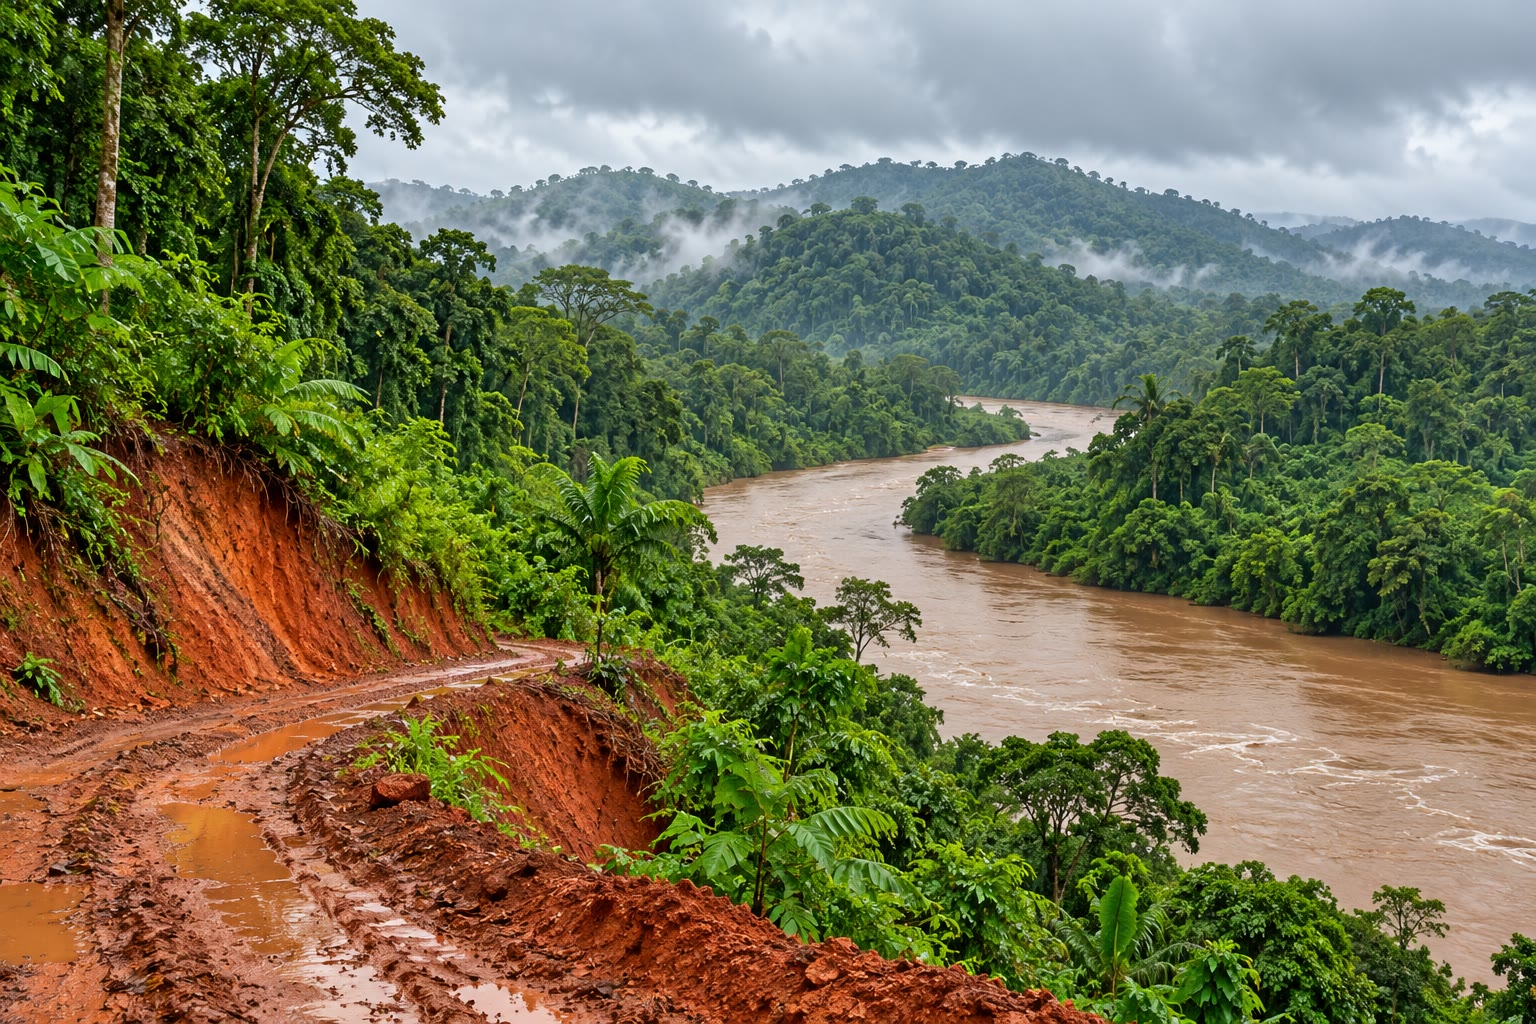
\includegraphics[width=0.66\linewidth]{images/book4/ai/b2-tropical-weathering.jpg}
\par\smallskip{\small Waar de thermostaat het hardst werkt: een heet, nat laagland, waar regen valt op
diep verweerde rode grond en de rivier de verweringsproducten naar zee voert
(door AI gegenereerde illustratie).}
\end{omfigure}

\section*{Oefeningen}\label{sec:b2:deep-time-climate:exercises}

Gegevens voor de oefeningen, tenzij anders vermeld: pre-industriële koolstof in de atmosfeer
\qty{591}{PgC} (\qty{278}{ppm}); $\qty{1}{Tmol}$ koolstof $= \qty{0.012011}{PgC}$;
silicaatverwering $W_0 = \qty{0.138}{PgC.yr^{-1}}$; aandeel van een overmaat dat na de oceaan en de
carbonaten in de lucht blijft $f = 0.08$; verweringsgevoeligheid $k_T = \qty{0.09}{K^{-1}}$; klimaatgevoeligheid $S =
\qty{3}{K}$; forcering van een verdubbeling van koolstofdioxide \qty{3.93}{W.m^{-2}}; $R =
\qty{8.314}{J.mol^{-1}.K^{-1}}$.
% ledger: ar6ch5:fig512, ipcc:erf-2xco2, derry24:fluxes, colbourn13:timescale, colbourn13:weathering, ipcc:ecs

\begin{exercise}[$\star$]\label{exo:b2:deep-time-climate:1}
Vóór het industriële tijdperk bevatte de oceaan \qty{900}{PgC} in haar oppervlaktelaag, \num{37100} in haar
intermediaire en diepe water, 700 als opgeloste organische koolstof en 3 in haar levende organismen.
(a) Hoeveel koolstof bevatte de oceaan, en hoeveel keer die van de atmosfeer? (b) Zet de
\qty{3.5e6}{Tmol} van de oppervlaktereservoirs om in petagram koolstof. (c) Welk aandeel daarvan zit in de
lucht?
\end{exercise}

\begin{exercise}[$\star$]\label{exo:b2:deep-time-climate:2}
Gebruik de fluxen van de figuur van de \omterm{def:b2:deep-time-climate:carbon-cycle}{koolstofcyclus op lange termijn}, met de metamorfe ontgassing gelijk aan
\qty{3}{Tmol.yr^{-1}}. (a) Tel de instroom naar de oppervlaktereservoirs en de uitstroom op.
(b) Welk aandeel van de instroom leveren vulkanen, riften en \omterm{def:b2:metamorphic-facies:metamorphism}{metamorfose}? (c) Bepaal de
verblijftijd van koolstof in de oppervlaktereservoirs, met behulp van de uitstroom.
\end{exercise}

\begin{exercise}[$\star$]\label{exo:b2:deep-time-climate:3}
(a) Schrijf de verwering van forsteriet, \ce{Mg2SiO4}, door koolstofdioxide en water tot magnesiumionen
en bicarbonaationen en opgelost silica, \ce{SiO2}, en maak de vergelijking kloppend. (b) Het magnesium wordt later
afgezet als carbonaat. Schrijf de nettoreactie. (c) Welke massa forsteriet moet verweren om
\qty{1}{PgC} voorgoed te verwijderen? ($M(\ce{Mg2SiO4}) = \qty{140.7}{g.mol^{-1}}$.)
\end{exercise}

\begin{exercise}[$\star$]\label{exo:b2:deep-time-climate:4}
Rangschik naar ouderdom, met hun datums, en zeg voor elk of de aarde in een broeikas- of
ijskasttoestand verkeerde: het Klimaatoptimum van het Vroeg-Eoceen; de Hirnantiaanse vergletsjering; het ontstaan van de
Antarctische ijskap; het Turonien; de grootste ijsuitbreiding van het late Paleozoïcum; de grote
opmarsen van de noordelijke ijskappen; het PETM.
\end{exercise}

\begin{exercise}[$\star\star$]\label{exo:b2:deep-time-climate:5}
(a) Ga na dat een activeringsenergie van \qty{63}{kJ.mol^{-1}} bij \qty{288}{K} $k_T =
\qty{0.09}{K^{-1}}$ geeft. (b) Bepaal $k_T$ voor de veldwaarde \qty{74}{kJ.mol^{-1}}. (c) Bepaal met elk
de stationaire opwarming wanneer de ontgassing met \qty{20}{\percent} stijgt. (d) Waarom komt de
klimaatgevoeligheid niet voor in (c)?
\end{exercise}

\begin{exercise}[$\star\star$]\label{exo:b2:deep-time-climate:6}
Vergelijk de exacte arrheniusfactor $\exp[-(E_{\text a}/R)(1/T - 1/T_0)]$ met $e^{k_T(T -
T_0)}$, $k_T = E_{\text a}/(RT_0^2)$, voor $E_{\text a} = \qty{63}{kJ.mol^{-1}}$ en $T_0 =
\qty{288}{K}$: (a) bij $T = \qty{293}{K}$; (b) bij $T = \qty{318}{K}$. (c) Toon aan dat de verhouding van de
benadering tot de exacte factor $\exp[E_{\text a}x^2/(RT_0^2(T_0 + x))]$ is, met $x = T - T_0$,
en bepaal de opwarming waarbij ze 1.1 bereikt.
\end{exercise}

\begin{exercise}[$\star\star$]\label{exo:b2:deep-time-climate:7}
De afgevlakte compilatie geeft \qty{1444}{ppm} koolstofdioxide bij \qty{419.5}{Ma} en
\qty{276}{ppm} aan het einde van haar reeks. (a) Bepaal de forcering van die daling. (b) Vergelijk ze met
de \qty{9}{W.m^{-2}} van de helderder wordende zon. (c) Bepaal de gemiddelde dalingssnelheid in ppm per miljoen
jaar, en vergelijk ze met de \qty{3.4}{ppm} van de aangepaste trend. Waarom kunnen ze verschillen?
\end{exercise}
% ledger: data:b4-foster2017, foster17:co2

\begin{exercise}[$\star\star$]\label{exo:b2:deep-time-climate:8}
(a) Spreid \num{3000} en \qty{7000}{PgC} over 3 en over \qty{20}{kyr}: welk bereik van
uitstootsnelheden volgt daaruit? Vergelijk met de 0.3 tot \qty{1.5}{PgC.yr^{-1}} die het IPCC opgeeft. (b) De menselijke uitstoot
bedroeg in 2010 ongeveer \qty{35}{Gt} koolstofdioxide. Zet om in koolstof en vergelijk. (c)
Koolstofdioxide steeg van 900 tot \qty{2000}{ppm}. Bepaal de forcering en de evenwichtsopwarming met $S =
\qty{3}{K}$, en vergelijk met de \qty{5}{\celsius} opwarming ten opzichte van het klimaat vóór het PETM.
\end{exercise}
% ledger: ar6ch5:petm-release, usgs:volcanic-co2, ar6ch5:petm

\begin{exercise}[$\star\star$]\label{exo:b2:deep-time-climate:9}
De opheffing van een gebergtegordel vermenigvuldigt de verweerbaarheid $W_0$ van de aarde met 1.2, bij een constante
ontgassing. (a) Bepaal de nieuwe stationaire temperatuurverandering. (b) Bepaal de nieuwe stationaire koolstofdioxide, vanaf
\qty{278}{ppm}. (c) Verschilt de snelheid van de silicaatverwering in de nieuwe stationaire toestand van de
oude? Leg uit.
\end{exercise}

\begin{exercise}[$\star\star\star$]\label{exo:b2:deep-time-climate:10}
(a) Bepaal de e-foldingtijd van de thermostaat met de afvoerfactor, $k = 0.09 + 0.65\times0.045$.
(b) Over miljoenen jaren reageren ook de ijskappen en de vegetatie; neem een
aardsysteemgevoeligheid van \qty{8}{K} per verdubbeling in plaats van $S$ en bepaal $\tau$ met $k_T$. (c) In welke richting duwen de
twee veranderingen de thermostaat, en welke onzekerheid, $E_{\text a}$ of $S$, weegt zwaarder?
\end{exercise}

\begin{exercise}[$\star\star\star$]\label{exo:b2:deep-time-climate:11}
Een uitstoot van \qty{5000}{PgC} (na de oceaan en de carbonaten). (a) Bepaal de koolstofdioxide van
de lucht, in ppm, en de opwarming. (b) Bepaal de aanvankelijke netto verwijderingssnelheid $W - W_0$, en de tijd die de
puls nodig zou hebben om met die snelheid te verdwijnen. (c) Bepaal de gelineariseerde tijd om \qty{90}{\percent}
van de overmaat te verwijderen. (d) Het model, zonder linearisering geïntegreerd, doet er \qty{340}{kyr} over. Waarom langer?
\end{exercise}

\begin{exercise}[$\star\star\star$]\label{exo:b2:deep-time-climate:12}
(a) Lineariseer het model rond een stationaire toestand waarin de ontgassing $V$ is en $C = C^*$, en toon aan dat
de e-foldingtijd $\tau' = A_0 (C^*/C_0)\ln 2/(f k S V)$ is. (b) Bereken ze voor de stationaire toestand
na een stijging van de ontgassing met \qty{20}{\percent}. (c) Is de thermostaat sneller of trager in een wereld die rijk is aan
koolstofdioxide, en waarom?
\end{exercise}

\begin{problem}[{Weekendprobleem --- Hoe lang doet de thermostaat erover?}]\label{pb:b2:deep-time-climate:1}
Dit probleem bouwt de tijdconstante van de thermostaat op uit gemeten fluxen. Gebruik de gegevens van de
oefeningen; ontgassing bij ruggen, \omterm{def:b2:oceanic-islands:stages}{oceaaneilanden}, bogen en riften \num{1.3}, \num{1.3}, 4.5 en
\qty{4.2}{Tmol.yr^{-1}}; silicaatverwering 11 tot \qty{12}{Tmol.yr^{-1}}; activeringsenergie
\qty{63}{kJ.mol^{-1}} bij $T_0 = \qty{288}{K}$; massa van de atmosfeer \qty{5.1e18}{kg}, gemiddelde molaire
massa van lucht \qty{28.97}{g.mol^{-1}}. Rond af op drie beduidende cijfers.

\noindent\textbf{Deel I --- Balans.}
\begin{enumerate}
  \item Tel de ontgassing van vulkanen en riften op, in \unit{Tmol.yr^{-1}} en in \unit{PgC.yr^{-1}}.
  \item Neem $W_0$ in het midden van zijn bereik; zet het om in \unit{PgC.yr^{-1}}.
  \item Vergelijk de twee. Wat suggereert de vergelijking over de \omterm{def:b2:deep-time-climate:carbon-cycle}{koolstofcyclus op lange termijn}?
  \item Hoeveel mol lucht bevat de atmosfeer? Hoeveel mol koolstof is \qty{591}{PgC},
        en welke mengverhouding is dat?
  \item Hoe lang zou de ontgassing van vraag 1 er zonder enige verwering over doen om
        \qty{591}{PgC} aan de oppervlaktereservoirs toe te voegen?
  \item Als een fractie $f = 0.08$ daarvan in de lucht bleef, met welke factor zou de
        koolstofdioxide van de lucht stijgen?
\end{enumerate}

\noindent\textbf{Deel II --- Lineariseren.}
\begin{enumerate}[resume]
  \item Bepaal $k_T$ uit de activeringsenergie, en ga na dat het afgerond de
        \qty{0.09}{K^{-1}} geeft die hieronder wordt gebruikt.
  \item Met welke factor groeit de verwering bij een opwarming van \qty{1}{K}?
  \item Schrijf de opwarming $\Delta T$ voor een overmaat $M$, en haar afgeleide bij $M = 0$, in
        \unit{K.PgC^{-1}}.
  \item Bepaal de afgeleide van $W$ naar $M$ bij $M = 0$, in \unit{yr^{-1}}.
  \item Toon aan dat haar inverse de tijdconstante $\tau$ van
        \cref{prop:b2:deep-time-climate:thermostat} is.
  \item Welke van $f$, $k$, $S$ en $W_0$ maken de thermostaat sneller wanneer ze toenemen?
\end{enumerate}

\noindent\textbf{Deel III --- De tijdconstante.}
\begin{enumerate}[resume]
  \item Bereken $\tau$.
  \item Bereken ze met de afvoerfactor, $k = \qty{0.119}{K^{-1}}$.
  \item Bereken ze met $k_T$ en een activeringsenergie van \qty{74}{kJ.mol^{-1}}.
  \item Vergelijk deze waarden met de \qty{200}{kyr} tot \qty{1}{Myr} van modellen met een expliciete oceaan.
  \item Hoeveel e-foldingtijden passen in de \qty{50}{Myr} van de cenozoïsche daling van
        koolstofdioxide? Wat zegt dat over de toestand van de koolstofcyclus tijdens de daling?
  \item Hoeveel verandert koolstofdioxide in één $\tau$, bij \qty{16}{ppm} per miljoen jaar?
\end{enumerate}

\noindent\textbf{Deel IV --- Een uitstoot ter grootte van het PETM.}
\begin{enumerate}[resume]
  \item Er komt \qty{5000}{PgC} vrij; hoeveel blijft er in de lucht nadat de oceaan en de carbonaten
        hun werk hebben gedaan, en wat is de koolstofdioxide in ppm?
  \item Bepaal de opwarming op dat moment.
  \item Hoeveel stijgt de verweringssnelheid, in \unit{PgC.yr^{-1}} en in procent?
  \item Hoe lang duurt het met de gelineariseerde wet tot \qty{90}{\percent} van de overmaat verdwenen is?
  \item Het carbonaat van het PETM herstelde zich over ongeveer \qty{100}{kyr}. Geef twee redenen waarom de echte
        aarde sneller kan zijn geweest dan dit model.
  \item Samengevat: wat is de e-foldingtijd van de \omterm{def:b2:deep-time-climate:thermostat}{silicaatverweringsthermostaat} in dit model?
\end{enumerate}
\end{problem}
% ledger: derry24:fluxes, colbourn13:weathering, colbourn13:timescale, ar6ch5:fig512, ar6ch5:petm, ar6ch5:cenozoic-co2, ipcc:ecs, earth:Matm, earth:Mmol
